\chapter{Appendix}
\label{appendix:Appendix}
\appendix




\section{Artificial Neural Networks}

An Artificial Neural Network or ANN is a computational model formed by a connection of artificial neurons arranged in structures called layers, \cite{ANN-graupe:2013}. Every ANN possesses three types of layers, the input layer, the hidden layer(s) and the output layer, see figure \ref{fig:ANN}.
\input{tikz/neural_network_tikz}

An artificial neuron, see figure \ref{fig:neuron}, is the simplest element of an ANN. Similar to a biological neuron, an artificial neuron has input connections through which it receives external stimuli, the input data $x$, \cite{ANN-graupe:2013}; With these inputs, the neuron makes a computation and generates an output value. This computation is a weighted sum of the input data where the weights $w$ are the parameters of the model that have to be adjusted in order for the model to learn. Furthermore, there is an additional input connection to the neuron, the parameter bias $b$ that also gets added to the weighted sum, $wx + b$. The final element of the artificial neuron is the activation function $f$ that takes as input the previous weighted sum and distorts it by adding non-linear deformations, $f(wx + b)$.

\input{tikz/neuron_tikz}

ANNs can be classified according to multiple taxonomies, one of them refers to the direction in which the data is propagated through the layers, giving as a result two main groups: feedforward neural networks (FNN) and recurrent neural networks (RNN), \cite{Classification-Artificial-Neural-Networks:2017}.

\subsection{Feedforward Neural Networks (FNNs)}

A feedworward neural network (FNN) is a type of artificial neural network where information flows in only one direction from the input layer to the output layer without going through any loop.
  \vspace{1mm} \\


\subsection{Recurrent Neural Networks (RNNs)}

Opposite to feedforward neural networks, recurrent neural networks (RNNs) propagate data both forwards and backwards through the layers endowing the model with memory. RNNs are specially useful when dealing with sequential or time dependent where some information underlays hidden, e.g., temporal information.

\vspace{5mm} 
\textbf{1. Vanilla RNN}

Vanilla RNNs are the simplest version of recurrent networks (Figure \ref{fig:rnn} shows an unrolled Vanilla RNN cell). The hidden state $h$ is a parameter whose dimension is defined by the user and it is this parameter $h$ the one that forms the recurrent connection within the cell. The hidden state at time $t$, $h_t$ is computed by adding the input data at that time, $x_t$, plus the hidden state from the previous time step $h_{t-1}$, see equation \ref{eq:vanilla_rnn}. It is precisely the fact of adding information from previous states, which makes the model able to remember.

%\input{rnn_tikz}

\begin{figure}[H]
    \centering
    \includegraphics[width=.7\textwidth]{Figures/rnn.png}
    \caption{Vanilla Recurrent Neural Network, \cite{Vanilla-RNN-image}}
    \label{fig:rnn}
\end{figure}



\begin{equation}
h_t=tanh(W_{xh}x_t+W_{hh}h_{t−1})
\end{equation}


\begin{equation}
h_t = tanh\left(\begin{pmatrix}
W_{xh} & W_{hh}
\end{pmatrix}
\begin{pmatrix}
x_t \\
h_{t−1} \\
\end{pmatrix}\right)
\label{eq:vanilla_rnn}
\end{equation}


Vanilla RNNs suffer from a problem called vanishing/exploding gradient that makes them unable to work properly with big temporal horizons. Here is where long short-term memory (LSTM) come to play.

\vspace{5mm} 
\textbf{2. Long Short-Term Memory (LSTM)}

LSTMs are an improved version of the Vanilla RNN; They are able to learn long term dependencies by maintaining not only the hidden state $h$ but also a cell state $c$ which is the key of these networks. Furthermore, an LSTM cell includes four gates that control the flow of information to the cell state.

\subsection{Convolutional Neural Networks (CNNs)}


A convolutional neural network is a special type of ANN mostly used when the input data are images from which we want to extract information. To achieve this, filters (also called kernels) convolve on the input data producing feature maps. An example of how this convolution is done, can be seen in figure \ref{fig:cnn}. The filter (blue) slides over the input image (red) and at every location, a matrix multiplication takes place giving as a result a feature map (green). The objective of these CNNs is to learn the filters in order to detect patterns in the input images.
\begin{figure}[H]
\centering
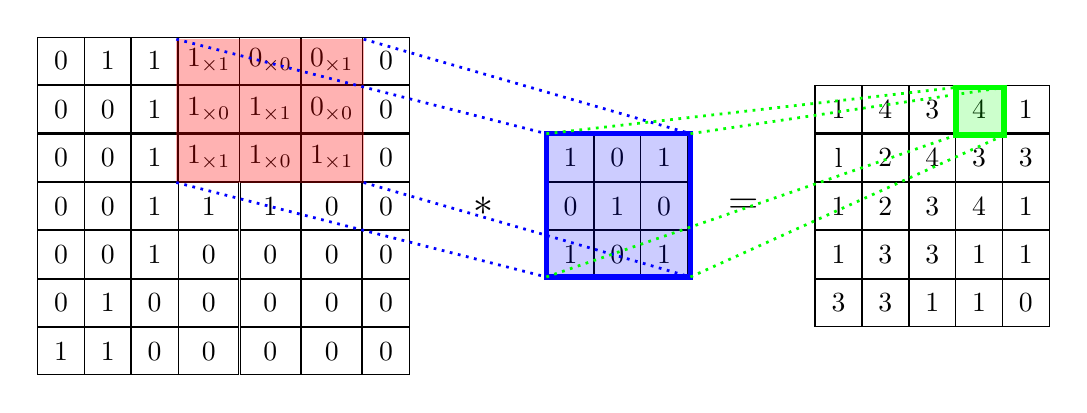
\begin{tikzpicture}[scale=1]

  \matrix [nodes=draw,column sep=-0.2mm, minimum size=6mm]
  {
    \node {0}; & \node{1}; & \node {1}; & \node{$1_{\times 1}$}; & \node{$0_{\times 0}$}; 
    & \node{$0_{\times 1}$}; & \node{0}; \\
    \node {0}; & \node{0}; & \node {1}; & \node{$1_{\times 0}$}; & \node{$1_{\times 1}$}; 
    & \node{$0_{\times 0}$}; & \node{0}; \\
    \node {0}; & \node{0}; & \node {1}; & \node{$1_{\times 1}$}; & \node{$1_{\times 0}$}; 
    & \node{$1_{\times 1}$}; & \node{0}; \\
    \node {0}; & \node{0}; & \node {1}; & \node{\, 1 \,}; & \node{\, 1 \, }; 
    & \node{\, 0 \,}; & \node{0}; \\
    \node {0}; & \node{0}; & \node {1}; & \node{\, 0 \, }; & \node{\, 0 \, }; 
    & \node{\, 0 \,}; & \node{0}; \\
    \node {0}; & \node{1}; & \node {0}; & \node{\, 0 \, }; & \node{\, 0 \, }; 
    & \node{\, 0 \,}; & \node{0}; \\
    \node {1}; & \node{1}; & \node {0}; & \node{\, 0 \,}; & \node{\, 0 \, }; 
    & \node{\, 0 \,}; & \node{0}; \\
  };


  % coordinates for coloring filter in array
  \coordinate (A) at (-0.6,0.3);
  \coordinate (B) at (1.78,0.3);
  \coordinate (C) at (1.78,2.12);
  \coordinate (D) at (-0.6,2.12);
  \fill[red, opacity=0.3] (A)--(B)--(C)--(D)--cycle;
  \begin{scope}[shift={(3.3,0)}]
    \node[] at (0,0) {\Large $\ast$};
  \end{scope}[shift={(2.5,0)}]

  \begin{scope}[shift={(5,0)}]

    %\matrix [matrix of math nodes,left delimiter={[},right
    %delimiter={]}]
    \matrix [nodes=draw,column sep=-0.2mm, minimum size=6mm]
    {
      \node{1};  & \node{0};   & \node{1};  \\
      \node{0};  & \node{1};   & \node{0};  \\
      \node{1}; & \node{0}; & \node{1}; \\
    };
    \coordinate (A1) at (-0.9,-0.9);
    \coordinate (B1) at (0.93,-0.9);
    \coordinate (C1) at (0.93,0.92);
    \coordinate (D1) at (-0.9,0.92);
    \fill[blue, opacity=0.2] (A1)--(B1)--(C1)--(D1)--cycle;
    \draw[blue, line width=2] (A1)--(B1)--(C1)--(D1)--cycle;
  \end{scope}

  \draw[dotted, line width=1, color=blue] (A)--(A1);
  \draw[dotted, line width=1, color=blue] (B)--(B1);
  \draw[dotted, line width=1, color=blue] (C)--(C1);
  \draw[dotted, line width=1, color=blue] (D)--(D1);

  \begin{scope}[shift={(6.6,0)}]
    \node[] at (0,0) {\Large $=$};
  \end{scope}[shift={(2.5,0)}]

  \begin{scope}[shift={(9,0)}]

    %\matrix [matrix of math nodes,left delimiter={[},right
    %delimiter={]}]
    \matrix [nodes=draw,column sep=-0.2mm, minimum size=6mm]
    {
      \node{1};  & \node{4};   & \node{3}; & \node{4}; & \node{1};  \\
      \node{l};  & \node{2};   & \node{4}; & \node{3}; & \node{3};  \\
      \node{1}; & \node{2}; & \node{3}; & \node{4} ; & \node{1};  \\
      \node{1}; & \node{3}; & \node{3}; & \node{1} ; & \node{1};  \\
      \node{3}; & \node{3}; & \node{1}; & \node{1} ; & \node{0};  \\
    };
    \coordinate (A2) at (0.3,0.9);
    \coordinate (B2) at (0.91,0.9);
    \coordinate (C2) at (0.91,1.507);
    \coordinate (D2) at (0.3,1.507);
    \fill[green, opacity=0.2] (A2)--(B2)--(C2)--(D2)--cycle;
    \draw[green, line width=2] (A2)--(B2)--(C2)--(D2)--cycle;
  \end{scope}

  \draw[dotted, line width=1, color=green] (A1)--(A2);
  \draw[dotted, line width=1, color=green] (B1)--(B2);
  \draw[dotted, line width=1, color=green] (C1)--(C2);
  \draw[dotted, line width=1, color=green] (D1)--(D2);
\end{tikzpicture}
\caption{Example of kernel in a CNN, \cite{Convolutional-tikz}} \label{fig:cnn}
\end{figure}








\subsection{Autoencoders}

An autoencoder, see figure \ref{fig:autoencoder} is neural network technique whose objective is to learn how to reduce the dimensionality of the input data, normally images, without losing their most important features. To do this, an autoencoder has three main parts: An encoder $e$, a latent space $L$ and a decoder $d$. The encoder $e(x)$, takes the input data and encodes it into a latent space $L$, a space of lower dimensionality. Then, the decoder takes this $L$ as input, and tries to reconstruct it so the output of the decoder is as similar as possible to the input $x$. The more similar is $\hat{x}$ to $x$, the better the relevant features have been captured into the latent space.

\begin{figure}[H]
\centering
\tikzset{arrow/.style={-stealth, thick, draw=gray!80!black}}

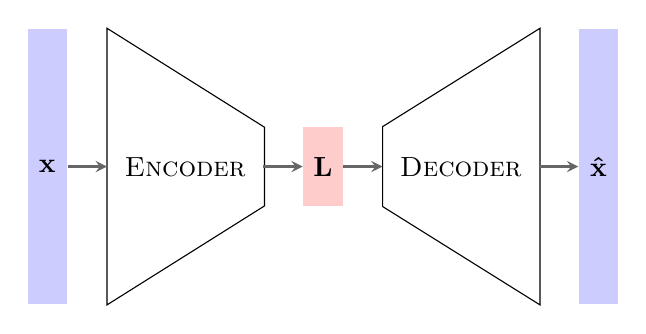
\begin{tikzpicture}
%     \draw[help lines](0,-5) grid (10,5);  
     
	\node[fill=blue!20, minimum width=0.5cm, minimum height=3.5cm] (X) at (0,0) {$\mathbf x$};
	
	\draw[fill=white!20] ([xshift=0.5cm]X.north east) -- ([xshift=2.5cm,yshift=0.5cm]X.east) -- ([xshift=2.5cm,yshift=-0.5cm]X.east) -- ([xshift=0.5cm]X.south east) -- cycle; 
	\node at (1.75,0) {\textsc{Encoder}};
	
	\node[fill=red!20, minimum width=0.5cm, minimum height=1.0cm] (Z) at (3.5cm,0) {$\mathbf L$};
	
	\draw[fill=white!20] ([xshift=0.5cm]Z.north east) -- ([xshift=2.5cm,yshift=1.25cm]Z.north east) -- ([xshift=2.5cm,yshift=-1.25cm]Z.south east) -- ([xshift=0.5cm]Z.south east) -- cycle;
	\node at (5.25,0) {\textsc{Decoder}};
	
	\node[fill=blue!20, minimum width=0.5cm, minimum height=3.5cm] (Xp) at (7,0) {$\mathbf{\hat{x}}$};
	
	\draw[arrow] (X.east) -- ([xshift=0.5cm]X.east);
	\draw[arrow] ([xshift=-0.5cm]Z.west) -- (Z.west);
	\draw[arrow] (Z.east) -- ([xshift=0.5cm]Z.east);
	\draw[arrow] ([xshift=-0.5cm]Xp.west) -- (Xp.west);
     
\end{tikzpicture}
\caption{Autoencoder, \cite{Autoencoder-tikz}} \label{fig:autoencoder}
\end{figure}
